%%%%%%%%%%%%%%%%%%%%%%%%%%%%%%%%%%%%%%%%%%%%%%%%%%%%%%%%%%%%
% 2.5 PROBABILISTIC NUMBER THEORY
% The Composition of Advanced Mathematics
%%%%%%%%%%%%%%%%%%%%%%%%%%%%%%%%%%%%%%%%%%%%%%%%%%%%%%%%%%%%

\section{Probabilistic Number Theory}
\label{sec:probabilistic-number-theory}

\prerequisite{
Elementary Number Theory from \cref{sec:elementary-number-theory}, especially
prime factorization, arithmetic functions, congruences, and the distribution
of primes. Basic probability, expectation, variance, and independence are
helpful. Formal probability theory is developed in Chapter 7.
}

\learningobjectives{
By the end of this section, the reader should be able to:
\begin{itemize}
    \item explain the probabilistic viewpoint in number theory;
    \item distinguish deterministic arithmetic statements from probabilistic models;
    \item interpret natural density as a notion of arithmetic frequency;
    \item compute densities of basic sets of integers;
    \item explain why divisibility by a prime can be modeled probabilistically;
    \item use heuristic independence of divisibility events appropriately;
    \item derive Euler products from probabilistic intuition;
    \item interpret arithmetic functions as random variables on finite integer sets;
    \item compute average orders of elementary arithmetic functions;
    \item distinguish average order from normal order;
    \item understand the typical size of the number of prime factors of an integer;
    \item distinguish \(\omega(n)\) and \(\Omega(n)\);
    \item state the Hardy--Ramanujan theorem conceptually;
    \item state and interpret the Erdős--Kac theorem;
    \item understand why \(\log\log n\) appears naturally in prime-factor statistics;
    \item study squarefree integers probabilistically;
    \item derive the density \(6/\pi^2\) of squarefree integers heuristically;
    \item understand the probabilistic behavior of coprimality;
    \item explain why two random integers are coprime with probability \(6/\pi^2\);
    \item understand probabilistic models for primes;
    \item explain the Cramér random model heuristically;
    \item distinguish rigorous probability statements from number-theoretic heuristics;
    \item understand additive arithmetic functions from a probabilistic perspective;
    \item recognize connections with analytic number theory, probability theory,
    combinatorics, and random structures.
\end{itemize}
}

%%%%%%%%%%%%%%%%%%%%%%%%%%%%%%%%%%%%%%%%%%%%%%%%%%%%%%%%%%%%
\subsection{What Is Probabilistic Number Theory?}
\label{subsec:what-is-probabilistic-number-theory}
%%%%%%%%%%%%%%%%%%%%%%%%%%%%%%%%%%%%%%%%%%%%%%%%%%%%%%%%%%%%

Number theory concerns deterministic objects.

An integer is either prime or composite.

A prime either divides an integer or it does not.

Yet when very large collections of integers are examined, arithmetic
properties often display statistical patterns.

\begin{definitionbox}{Probabilistic Number Theory}
\emph{Probabilistic number theory} studies the statistical distribution of
arithmetic properties and uses ideas from probability theory to understand
the typical behavior of integers and arithmetic functions.
\end{definitionbox}

Typical questions include:

\begin{itemize}
    \item What proportion of integers are squarefree?
    \item How many prime factors does a typical integer have?
    \item What proportion of pairs of integers are coprime?
    \item How are values of arithmetic functions distributed?
    \item Can primes be approximated by a random model?
\end{itemize}

The guiding viewpoint is

\[
\boxed{
\text{integers are deterministic individually but statistical collectively}.
}
\]

%%%%%%%%%%%%%%%%%%%%%%%%%%%%%%%%%%%%%%%%%%%%%%%%%%%%%%%%%%%%
\subsection{Choosing a Random Integer}
\label{subsec:choosing-random-integer}
%%%%%%%%%%%%%%%%%%%%%%%%%%%%%%%%%%%%%%%%%%%%%%%%%%%%%%%%%%%%

There is no uniform probability distribution on all positive integers in
which every integer receives the same positive probability.

Instead, choose an integer uniformly from

\[ \{1,2,\ldots,N\} \]

and study what happens as

\[ N\to\infty. \]

For an arithmetic property \(P\), define

\[ \Pr_N(P)=\frac{\#\{n\leq N:n\text{ satisfies }P\}}{N}. \]

The symbol

\[ \Pr_N(P) \]

is read ``the probability of \(P\) up to \(N\).''

If this quantity approaches a limit, that limit gives a natural notion of
density.

%%%%%%%%%%%%%%%%%%%%%%%%%%%%%%%%%%%%%%%%%%%%%%%%%%%%%%%%%%%%
\subsection{Natural Density}
\label{subsec:natural-density}
%%%%%%%%%%%%%%%%%%%%%%%%%%%%%%%%%%%%%%%%%%%%%%%%%%%%%%%%%%%%

\begin{definitionbox}{Natural Density}
Let \(A\subseteq\N\). If the limit

\[ d(A)=\lim_{N\to\infty}\frac{\#(A\cap\{1,\ldots,N\})}{N} \]

exists, it is called the \emph{natural density} of \(A\).
\end{definitionbox}

The notation

\[ d(A) \]

is read ``the density of \(A\).''

It measures the asymptotic proportion of positive integers belonging to
\(A\).

%%%%%%%%%%%%%%%%%%%%%%%%%%%%%%%%%%%%%%%%%%%%%%%%%%%%%%%%%%%%
\subsection{Example: Density of Even Integers}
\label{subsec:density-even-integers}
%%%%%%%%%%%%%%%%%%%%%%%%%%%%%%%%%%%%%%%%%%%%%%%%%%%%%%%%%%%%

Among the first \(N\) positive integers, approximately half are even.

Thus

\[ \boxed{d(2\Z_{>0})=\frac12.} \]

Likewise, the multiples of a positive integer \(m\) have density

\[ \boxed{\frac1m.} \]

This simple observation becomes a basic probabilistic model for divisibility.

%%%%%%%%%%%%%%%%%%%%%%%%%%%%%%%%%%%%%%%%%%%%%%%%%%%%%%%%%%%%
\subsection{Divisibility as an Event}
\label{subsec:divisibility-as-event}
%%%%%%%%%%%%%%%%%%%%%%%%%%%%%%%%%%%%%%%%%%%%%%%%%%%%%%%%%%%%

Fix a prime \(p\).

The multiples of \(p\) have density

\[ \frac1p. \]

Thus, for a large randomly selected integer \(n\), it is natural to write
heuristically

\[ \boxed{\Pr(p\mid n)\approx\frac1p.} \]

Similarly,

\[ \Pr(p\nmid n)\approx1-\frac1p. \]

For divisibility by \(p^k\),

\[ \boxed{\Pr(p^k\mid n)\approx\frac1{p^k}.} \]

%%%%%%%%%%%%%%%%%%%%%%%%%%%%%%%%%%%%%%%%%%%%%%%%%%%%%%%%%%%%
\subsection{A Divisibility Probability Tree}
\label{subsec:divisibility-probability-tree}
%%%%%%%%%%%%%%%%%%%%%%%%%%%%%%%%%%%%%%%%%%%%%%%%%%%%%%%%%%%%

\begin{centereddiagram}
\begin{tikzpicture}[
    level distance=14mm,
    level 1/.style={sibling distance=50mm},
    level 2/.style={sibling distance=24mm},
    every node/.style={align=center},
    edge from parent/.style={-{Latex[length=2.3mm]}}
]
\node {\(n\)}
child {node {\(p\mid n\)}
    edge from parent node[left] {\(\frac1p\)}
    child {node {\(p^2\mid n\)}
        edge from parent node[left] {\(\frac1p\)}}
    child {node {\(p^2\nmid n\)}
        edge from parent node[right] {\(1-\frac1p\)}}}
child {node {\(p\nmid n\)}
    edge from parent node[right] {\(1-\frac1p\)}};
\end{tikzpicture}
\end{centereddiagram}

Conditional on \(p\mid n\), the heuristic probability of another factor of
\(p\) is again approximately \(1/p\).

%%%%%%%%%%%%%%%%%%%%%%%%%%%%%%%%%%%%%%%%%%%%%%%%%%%%%%%%%%%%
\subsection{Divisibility by Distinct Primes}
\label{subsec:distinct-prime-divisibility}
%%%%%%%%%%%%%%%%%%%%%%%%%%%%%%%%%%%%%%%%%%%%%%%%%%%%%%%%%%%%

Let \(p\neq q\) be primes.

The integers divisible by both \(p\) and \(q\) are precisely the multiples of

\[ pq. \]

Therefore their density is

\[ \frac1{pq}. \]

But

\[ \frac1{pq}=\frac1p\frac1q. \]

Thus the events

\[ p\mid n \]

and

\[ q\mid n \]

behave like independent events in the limiting density model.

%%%%%%%%%%%%%%%%%%%%%%%%%%%%%%%%%%%%%%%%%%%%%%%%%%%%%%%%%%%%
\subsection{Arithmetic Independence}
\label{subsec:arithmetic-independence}
%%%%%%%%%%%%%%%%%%%%%%%%%%%%%%%%%%%%%%%%%%%%%%%%%%%%%%%%%%%%

For distinct primes

\[ p_1,\ldots,p_r, \]

the Chinese Remainder Theorem implies that divisibility conditions modulo
their powers combine cleanly.

For example,

\[
\Pr(p_1\mid n,\ldots,p_r\mid n)
\approx
\frac1{p_1\cdots p_r}.
\]

This equals

\[ \prod_{j=1}^{r}\frac1{p_j}. \]

\begin{conceptbox}
Distinct-prime divisibility behaves like independence because congruence
conditions modulo coprime moduli combine through the Chinese Remainder
Theorem.
\end{conceptbox}

This observation is one of the foundations of probabilistic number theory.

%%%%%%%%%%%%%%%%%%%%%%%%%%%%%%%%%%%%%%%%%%%%%%%%%%%%%%%%%%%%
\subsection{Important Limitation of the Independence Model}
\label{subsec:independence-model-limitation}
%%%%%%%%%%%%%%%%%%%%%%%%%%%%%%%%%%%%%%%%%%%%%%%%%%%%%%%%%%%%

Divisibility events are not literally independent in every finite model.

For example, if

\[ p>N, \]

then no integer in

\[ \{1,\ldots,N\} \]

is divisible by \(p\).

Furthermore, an integer \(n\leq N\) cannot be divisible by too many very
large primes simultaneously.

Thus independence is often an asymptotic approximation rather than a literal
finite statement.

\begin{warningbox}
Probabilistic models in number theory must be distinguished from rigorous
probability spaces.

A heuristic can predict the correct answer without itself constituting a
proof.
\end{warningbox}

%%%%%%%%%%%%%%%%%%%%%%%%%%%%%%%%%%%%%%%%%%%%%%%%%%%%%%%%%%%%
\subsection{Euler Products as Probability Products}
\label{subsec:euler-products-probability}
%%%%%%%%%%%%%%%%%%%%%%%%%%%%%%%%%%%%%%%%%%%%%%%%%%%%%%%%%%%%

The probability that a large integer is not divisible by a prime \(p\) is
approximately

\[ 1-\frac1p. \]

If prime divisibility is treated as independent, the probability that an
integer is divisible by no prime at all would suggest the product

\[ \prod_p\left(1-\frac1p\right). \]

The product tends to zero, consistent with the fact that every integer
greater than \(1\) has a prime divisor.

More generally, products over primes arise naturally whenever arithmetic
conditions are decomposed prime by prime.

This probabilistic viewpoint parallels Euler products in analytic number
theory.

%%%%%%%%%%%%%%%%%%%%%%%%%%%%%%%%%%%%%%%%%%%%%%%%%%%%%%%%%%%%
\subsection{Squarefree Integers}
\label{subsec:probabilistic-squarefree-integers}
%%%%%%%%%%%%%%%%%%%%%%%%%%%%%%%%%%%%%%%%%%%%%%%%%%%%%%%%%%%%

Recall that an integer \(n\) is squarefree if no prime square divides it.

Thus

\[ n\text{ squarefree}\quad\Longleftrightarrow\quad p^2\nmid n \]

for every prime \(p\).

For a fixed prime,

\[ \Pr(p^2\mid n)\approx\frac1{p^2}. \]

Hence

\[ \Pr(p^2\nmid n)\approx1-\frac1{p^2}. \]

Assuming the prime-square conditions behave independently suggests

\[ \Pr(n\text{ squarefree})\approx\prod_p\left(1-\frac1{p^2}\right). \]

%%%%%%%%%%%%%%%%%%%%%%%%%%%%%%%%%%%%%%%%%%%%%%%%%%%%%%%%%%%%
\subsection{Density of Squarefree Integers}
\label{subsec:density-squarefree}
%%%%%%%%%%%%%%%%%%%%%%%%%%%%%%%%%%%%%%%%%%%%%%%%%%%%%%%%%%%%

Euler's product for the Riemann zeta function gives

\[ \frac1{\zeta(s)}=\prod_p\left(1-\frac1{p^s}\right). \]

Setting \(s=2\),

\[ \prod_p\left(1-\frac1{p^2}\right)=\frac1{\zeta(2)}. \]

Since

\[ \zeta(2)=\frac{\pi^2}{6}, \]

we obtain

\[ \boxed{d(\text{squarefree integers})=\frac6{\pi^2}.} \]

Numerically,

\[ \frac6{\pi^2}\approx0.6079. \]

Thus about \(60.8\%\) of positive integers are squarefree.

%%%%%%%%%%%%%%%%%%%%%%%%%%%%%%%%%%%%%%%%%%%%%%%%%%%%%%%%%%%%
\subsection{Squarefree Density Visual}
\label{subsec:squarefree-density-visual}
%%%%%%%%%%%%%%%%%%%%%%%%%%%%%%%%%%%%%%%%%%%%%%%%%%%%%%%%%%%%

\begin{centereddiagram}
\begin{tikzpicture}[x=0.34cm,y=0.55cm]
\foreach \n in {1,...,30}{
    \pgfmathtruncatemacro{\row}{int((\n-1)/10)}
    \pgfmathtruncatemacro{\col}{mod(\n-1,10)}
    \node[draw,minimum width=0.62cm,minimum height=0.48cm] (n\n)
    at (\col*2,-\row) {\scriptsize \n};
}
\foreach \n in {1,2,3,5,6,7,10,11,13,14,15,17,19,21,22,23,26,29,30}{
    \node[draw=MathBlue,line width=0.9pt,rounded corners,
    fit=(n\n),inner sep=0pt] {};
}
\end{tikzpicture}
\end{centereddiagram}

The highlighted integers are squarefree.

The proportion fluctuates for small ranges but approaches

\[ \frac6{\pi^2} \]

as the range grows.

%%%%%%%%%%%%%%%%%%%%%%%%%%%%%%%%%%%%%%%%%%%%%%%%%%%%%%%%%%%%
\subsection{Coprime Pairs}
\label{subsec:probabilistic-coprime-pairs}
%%%%%%%%%%%%%%%%%%%%%%%%%%%%%%%%%%%%%%%%%%%%%%%%%%%%%%%%%%%%

Choose two large integers \(a\) and \(b\).

They fail to be coprime precisely when some prime divides both.

For a fixed prime \(p\),

\[ \Pr(p\mid a)\approx\frac1p,\qquad \Pr(p\mid b)\approx\frac1p. \]

Treating the choices independently,

\[ \Pr(p\mid a\text{ and }p\mid b)\approx\frac1{p^2}. \]

Therefore the probability that \(p\) does not divide both is

\[ 1-\frac1{p^2}. \]

Multiplying over all primes suggests

\[ \Pr(\gcd(a,b)=1)=\prod_p\left(1-\frac1{p^2}\right). \]

Hence

\[ \boxed{\Pr(\gcd(a,b)=1)=\frac6{\pi^2}.} \]

%%%%%%%%%%%%%%%%%%%%%%%%%%%%%%%%%%%%%%%%%%%%%%%%%%%%%%%%%%%%
\subsection{A Surprising Coincidence}
\label{subsec:squarefree-coprime-coincidence}
%%%%%%%%%%%%%%%%%%%%%%%%%%%%%%%%%%%%%%%%%%%%%%%%%%%%%%%%%%%%

The same constant

\[ \frac6{\pi^2} \]

appears in two different questions:

\[
\boxed{
\Pr(n\text{ is squarefree})
=
\Pr(\gcd(a,b)=1)
=
\frac6{\pi^2}.
}
\]

This happens because both conditions produce the same local factor

\[ 1-\frac1{p^2} \]

for every prime \(p\).

This is a common phenomenon in multiplicative number theory.

%%%%%%%%%%%%%%%%%%%%%%%%%%%%%%%%%%%%%%%%%%%%%%%%%%%%%%%%%%%%
\subsection{Coprimality of Several Integers}
\label{subsec:coprimality-several-integers}
%%%%%%%%%%%%%%%%%%%%%%%%%%%%%%%%%%%%%%%%%%%%%%%%%%%%%%%%%%%%

Choose \(k\) integers independently from a large range.

The probability that a fixed prime \(p\) divides all \(k\) integers is

\[ \frac1{p^k}. \]

Therefore the probability that their greatest common divisor equals \(1\) is

\[
\boxed{
\Pr(\gcd(n_1,\ldots,n_k)=1)
=
\prod_p\left(1-\frac1{p^k}\right)
=
\frac1{\zeta(k)}.
}
\]

For \(k=2\), this becomes

\[ \frac1{\zeta(2)}=\frac6{\pi^2}. \]

%%%%%%%%%%%%%%%%%%%%%%%%%%%%%%%%%%%%%%%%%%%%%%%%%%%%%%%%%%%%
\subsection{Arithmetic Functions as Random Variables}
\label{subsec:arithmetic-functions-random-variables}
%%%%%%%%%%%%%%%%%%%%%%%%%%%%%%%%%%%%%%%%%%%%%%%%%%%%%%%%%%%%

Fix \(N\) and choose

\[ n\in\{1,\ldots,N\} \]

uniformly.

Any arithmetic function

\[ f:\N\to\R \]

can then be regarded as a random variable

\[ f(n). \]

Its finite average is

\[ \boxed{\frac1N\sum_{n\leq N}f(n).} \]

This quantity plays the role of an expectation.

%%%%%%%%%%%%%%%%%%%%%%%%%%%%%%%%%%%%%%%%%%%%%%%%%%%%%%%%%%%%
\subsection{Average Order}
\label{subsec:average-order}
%%%%%%%%%%%%%%%%%%%%%%%%%%%%%%%%%%%%%%%%%%%%%%%%%%%%%%%%%%%%

\begin{definitionbox}{Average Order}
An arithmetic function \(g(n)\) is an \emph{average order} of \(f(n)\) if,
in an appropriate asymptotic sense,

\[ \sum_{n\leq x}f(n)\sim\sum_{n\leq x}g(n). \]
\end{definitionbox}

The symbol

\[ \sim \]

is read ``is asymptotic to.''

It means the ratio of the two quantities approaches \(1\).

An average order describes the aggregate behavior of an arithmetic function,
not necessarily its value at a typical individual integer.

%%%%%%%%%%%%%%%%%%%%%%%%%%%%%%%%%%%%%%%%%%%%%%%%%%%%%%%%%%%%
\subsection{Example: Average Number of Divisors}
\label{subsec:average-number-divisors}
%%%%%%%%%%%%%%%%%%%%%%%%%%%%%%%%%%%%%%%%%%%%%%%%%%%%%%%%%%%%

Let

\[ \tau(n) \]

denote the number of positive divisors of \(n\).

Then

\[
\sum_{n\leq x}\tau(n)
=
\sum_{n\leq x}\sum_{d\mid n}1.
\]

Reverse the order of counting:

\[
\sum_{n\leq x}\tau(n)
=
\sum_{d\leq x}\left\lfloor\frac{x}{d}\right\rfloor.
\]

Since

\[ \left\lfloor\frac{x}{d}\right\rfloor\approx\frac{x}{d}, \]

we expect

\[
\sum_{n\leq x}\tau(n)
\approx
x\sum_{d\leq x}\frac1d.
\]

The harmonic sum behaves like

\[ \log x. \]

Thus

\[ \boxed{\tau(n)\text{ has average order approximately }\log n.} \]

A more precise result includes lower-order terms.

%%%%%%%%%%%%%%%%%%%%%%%%%%%%%%%%%%%%%%%%%%%%%%%%%%%%%%%%%%%%
\subsection{Average Order Versus Typical Size}
\label{subsec:average-versus-typical}
%%%%%%%%%%%%%%%%%%%%%%%%%%%%%%%%%%%%%%%%%%%%%%%%%%%%%%%%%%%%

Average order and typical behavior are different ideas.

A small number of unusually large values can strongly affect an average.

For example, an arithmetic function may have average order \(g(n)\) even
though most individual values are not especially close to \(g(n)\).

This motivates the notion of normal order.

%%%%%%%%%%%%%%%%%%%%%%%%%%%%%%%%%%%%%%%%%%%%%%%%%%%%%%%%%%%%
\subsection{Normal Order}
\label{subsec:normal-order}
%%%%%%%%%%%%%%%%%%%%%%%%%%%%%%%%%%%%%%%%%%%%%%%%%%%%%%%%%%%%

\begin{definitionbox}{Normal Order}
A positive function \(g(n)\) is a \emph{normal order} of an arithmetic
function \(f(n)\) if, for every \(\varepsilon>0\), the proportion of integers
\(n\leq x\) satisfying

\[ |f(n)-g(n)|>\varepsilon g(n) \]

tends to \(0\) as

\[ x\to\infty. \]
\end{definitionbox}

Thus

\[ f(n)\approx g(n) \]

for almost all integers in the density sense.

%%%%%%%%%%%%%%%%%%%%%%%%%%%%%%%%%%%%%%%%%%%%%%%%%%%%%%%%%%%%
\subsection{Counting Distinct Prime Factors}
\label{subsec:omega-distinct-prime-factors}
%%%%%%%%%%%%%%%%%%%%%%%%%%%%%%%%%%%%%%%%%%%%%%%%%%%%%%%%%%%%

Define

\[ \omega(n)=\#\{p:p\mid n\}. \]

The Greek letter

\[ \omega \]

is lowercase \emph{omega}, pronounced ``oh-MAY-guh.''

The function \(\omega(n)\) counts the number of \emph{distinct} prime factors
of \(n\).

For example,

\[ 60=2^2\cdot3\cdot5, \]

so

\[ \boxed{\omega(60)=3.} \]

%%%%%%%%%%%%%%%%%%%%%%%%%%%%%%%%%%%%%%%%%%%%%%%%%%%%%%%%%%%%
\subsection{Counting Prime Factors with Multiplicity}
\label{subsec:big-omega-prime-factors}
%%%%%%%%%%%%%%%%%%%%%%%%%%%%%%%%%%%%%%%%%%%%%%%%%%%%%%%%%%%%

Define

\[ \Omega(n) \]

to be the number of prime factors counted with multiplicity.

The symbol

\[ \Omega \]

is uppercase \emph{omega}.

If

\[ n=p_1^{e_1}\cdots p_r^{e_r}, \]

then

\[ \boxed{\Omega(n)=e_1+\cdots+e_r.} \]

For

\[ 60=2^2\cdot3\cdot5, \]

we have

\[ \boxed{\Omega(60)=4.} \]

Thus

\[ \omega(60)=3,\qquad\Omega(60)=4. \]

%%%%%%%%%%%%%%%%%%%%%%%%%%%%%%%%%%%%%%%%%%%%%%%%%%%%%%%%%%%%
\subsection{Prime-Factor Indicators}
\label{subsec:prime-factor-indicators}
%%%%%%%%%%%%%%%%%%%%%%%%%%%%%%%%%%%%%%%%%%%%%%%%%%%%%%%%%%%%

For each prime \(p\), define

\[
X_p(n)=
\begin{cases}
1, & p\mid n,\\
0, & p\nmid n.
\end{cases}
\]

Then

\[ \boxed{\omega(n)=\sum_{p\mid n}1=\sum_{p\leq n}X_p(n).} \]

Heuristically,

\[ \Pr(X_p=1)\approx\frac1p. \]

Therefore

\[ \Expect[X_p]\approx\frac1p. \]

The symbol

\[ \Expect \]

is read ``expected value.''

This notation is developed formally in Probability Theory.

%%%%%%%%%%%%%%%%%%%%%%%%%%%%%%%%%%%%%%%%%%%%%%%%%%%%%%%%%%%%
\subsection{Expected Number of Distinct Prime Factors}
\label{subsec:expected-distinct-prime-factors}
%%%%%%%%%%%%%%%%%%%%%%%%%%%%%%%%%%%%%%%%%%%%%%%%%%%%%%%%%%%%

Using linearity of expectation,

\[
\Expect[\omega(n)]
\approx
\sum_{p\leq n}\frac1p.
\]

A classical result states

\[ \sum_{p\leq x}\frac1p=\log\log x+O(1). \]

Therefore

\[ \boxed{\Expect[\omega(n)]\approx\log\log n.} \]

This explains the appearance of the slowly growing quantity

\[ \log\log n. \]

%%%%%%%%%%%%%%%%%%%%%%%%%%%%%%%%%%%%%%%%%%%%%%%%%%%%%%%%%%%%
\subsection{How Slowly Does \(\log\log n\) Grow?}
\label{subsec:log-log-growth}
%%%%%%%%%%%%%%%%%%%%%%%%%%%%%%%%%%%%%%%%%%%%%%%%%%%%%%%%%%%%

The function

\[ \log\log n \]

grows extremely slowly.

For illustration,

\[
\begin{array}{c|c}
n & \log\log n\\
\hline
10^3 & \approx1.93\\
10^6 & \approx2.63\\
10^{12} & \approx3.32\\
10^{100} & \approx5.44
\end{array}
\]

where natural logarithms are used.

Thus even extraordinarily large integers typically have a surprisingly
modest number of distinct prime factors.

%%%%%%%%%%%%%%%%%%%%%%%%%%%%%%%%%%%%%%%%%%%%%%%%%%%%%%%%%%%%
\subsection{Hardy--Ramanujan Theorem}
\label{subsec:hardy-ramanujan-theorem}
%%%%%%%%%%%%%%%%%%%%%%%%%%%%%%%%%%%%%%%%%%%%%%%%%%%%%%%%%%%%

The probabilistic prediction is not merely heuristic.

\begin{theorem}[Hardy--Ramanujan]
For almost all positive integers \(n\),

\[ \boxed{\omega(n)\sim\log\log n} \]

in the normal-order sense.

Likewise,

\[ \boxed{\Omega(n)\sim\log\log n} \]

for almost all \(n\).
\end{theorem}

The phrase \emph{almost all integers} means that the proportion of exceptions
among

\[ 1,\ldots,N \]

tends to zero as

\[ N\to\infty. \]

%%%%%%%%%%%%%%%%%%%%%%%%%%%%%%%%%%%%%%%%%%%%%%%%%%%%%%%%%%%%
\subsection{A Probabilistic Interpretation}
\label{subsec:hardy-ramanujan-probabilistic}
%%%%%%%%%%%%%%%%%%%%%%%%%%%%%%%%%%%%%%%%%%%%%%%%%%%%%%%%%%%%

Think of

\[ \omega(n)=\sum_p X_p(n) \]

as a sum of approximately independent Bernoulli-type variables, where

\[ \Pr(X_p=1)\approx\frac1p. \]

The expected value is approximately

\[ \sum_{p\leq n}\frac1p\approx\log\log n. \]

Thus probability predicts that the number of prime factors should cluster
around

\[ \log\log n. \]

Hardy and Ramanujan established this concentration rigorously.

%%%%%%%%%%%%%%%%%%%%%%%%%%%%%%%%%%%%%%%%%%%%%%%%%%%%%%%%%%%%
\subsection{Variance Heuristic}
\label{subsec:omega-variance}
%%%%%%%%%%%%%%%%%%%%%%%%%%%%%%%%%%%%%%%%%%%%%%%%%%%%%%%%%%%%

For a Bernoulli variable with success probability \(1/p\),

\[ \Var(X_p)\approx\frac1p\left(1-\frac1p\right). \]

The notation

\[ \Var(X_p) \]

is read ``the variance of \(X_p\).''

Assuming approximate independence,

\[
\Var(\omega(n))
\approx
\sum_{p\leq n}
\frac1p\left(1-\frac1p\right).
\]

The dominant term is again

\[ \log\log n. \]

Thus the standard deviation should be approximately

\[ \sqrt{\log\log n}. \]

%%%%%%%%%%%%%%%%%%%%%%%%%%%%%%%%%%%%%%%%%%%%%%%%%%%%%%%%%%%%
\subsection{Erdős--Kac Theorem}
\label{subsec:erdos-kac-theorem}
%%%%%%%%%%%%%%%%%%%%%%%%%%%%%%%%%%%%%%%%%%%%%%%%%%%%%%%%%%%%

The prime-factor count behaves even more like a classical random variable
than the Hardy--Ramanujan theorem suggests.

\begin{theorem}[Erdős--Kac]
As \(n\) ranges over the positive integers, the normalized quantity

\[
\boxed{
\frac{\omega(n)-\log\log n}{\sqrt{\log\log n}}
}
\]

approaches the standard normal distribution.
\end{theorem}

In other words, the number of distinct prime factors of a typical integer
has approximately:

\[
\text{mean}\approx\log\log n,
\qquad
\text{variance}\approx\log\log n.
\]

%%%%%%%%%%%%%%%%%%%%%%%%%%%%%%%%%%%%%%%%%%%%%%%%%%%%%%%%%%%%
\subsection{The Gaussian Shape}
\label{subsec:erdos-kac-gaussian-visual}
%%%%%%%%%%%%%%%%%%%%%%%%%%%%%%%%%%%%%%%%%%%%%%%%%%%%%%%%%%%%

The standard normal density is

\[ \phi(x)=\frac1{\sqrt{2\pi}}e^{-x^2/2}. \]

Here

\[ \phi \]

is lowercase Greek \emph{phi}, commonly pronounced ``fie'' or ``fee''
depending on convention.

\begin{centereddiagram}
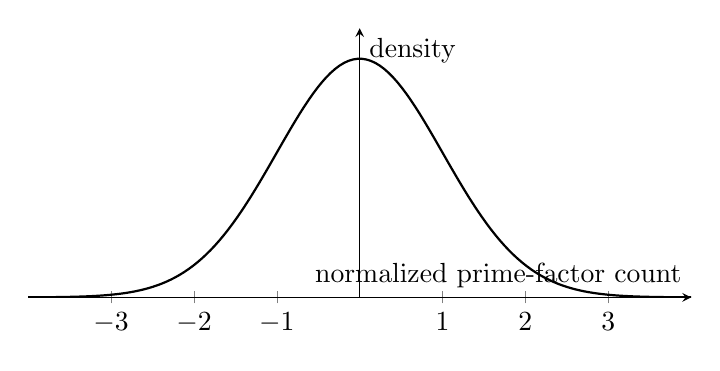
\begin{tikzpicture}
\begin{axis}[
    width=10cm,
    height=5cm,
    axis lines=middle,
    xmin=-4,xmax=4,
    ymin=0,ymax=0.45,
    xlabel={normalized prime-factor count},
    ylabel={density},
    samples=150,
    domain=-4:4,
    xtick={-3,-2,-1,0,1,2,3},
    ytick=\empty
]
\addplot[thick] {1/sqrt(2*pi)*exp(-x^2/2)};
\end{axis}
\end{tikzpicture}
\end{centereddiagram}

The Erdős--Kac theorem says that the normalized distribution of
\(\omega(n)\) approaches this bell-shaped curve.

%%%%%%%%%%%%%%%%%%%%%%%%%%%%%%%%%%%%%%%%%%%%%%%%%%%%%%%%%%%%
\subsection{Why Erdős--Kac Is Remarkable}
\label{subsec:why-erdos-kac-remarkable}
%%%%%%%%%%%%%%%%%%%%%%%%%%%%%%%%%%%%%%%%%%%%%%%%%%%%%%%%%%%%

The central limit theorem usually concerns sums of random variables.

But

\[ \omega(n) \]

is a deterministic arithmetic function.

Nevertheless, when integers are sampled from increasingly large intervals,
its distribution behaves like the sum of many weakly dependent random
variables.

\begin{importantbox}
The Erdős--Kac theorem is one of the clearest demonstrations that deterministic
arithmetic structures can exhibit genuine statistical laws.
\end{importantbox}

%%%%%%%%%%%%%%%%%%%%%%%%%%%%%%%%%%%%%%%%%%%%%%%%%%%%%%%%%%%%
\subsection{Additive Arithmetic Functions}
\label{subsec:additive-arithmetic-functions-probabilistic}
%%%%%%%%%%%%%%%%%%%%%%%%%%%%%%%%%%%%%%%%%%%%%%%%%%%%%%%%%%%%

\begin{definitionbox}{Additive Arithmetic Function}
An arithmetic function \(f\) is \emph{additive} if

\[ f(mn)=f(m)+f(n) \]

whenever

\[ \gcd(m,n)=1. \]
\end{definitionbox}

Both

\[ \omega(n) \]

and

\[ \Omega(n) \]

are additive.

For example, if

\[ \gcd(m,n)=1, \]

then the distinct prime factors of \(mn\) are precisely the prime factors of
\(m\) together with those of \(n\).

Hence

\[ \omega(mn)=\omega(m)+\omega(n). \]

%%%%%%%%%%%%%%%%%%%%%%%%%%%%%%%%%%%%%%%%%%%%%%%%%%%%%%%%%%%%
\subsection{Strongly Additive Functions}
\label{subsec:strongly-additive-functions}
%%%%%%%%%%%%%%%%%%%%%%%%%%%%%%%%%%%%%%%%%%%%%%%%%%%%%%%%%%%%

\begin{definitionbox}{Strongly Additive Function}
An additive function \(f\) is \emph{strongly additive} if

\[ f(p^k)=f(p) \]

for every prime \(p\) and every integer \(k\geq1\).
\end{definitionbox}

The function

\[ \omega(n) \]

is strongly additive because the exponent of a prime does not affect whether
that prime is counted.

By contrast,

\[ \Omega(p^k)=k, \]

so \(\Omega\) is additive but not strongly additive.

%%%%%%%%%%%%%%%%%%%%%%%%%%%%%%%%%%%%%%%%%%%%%%%%%%%%%%%%%%%%
\subsection{Probabilistic Model for Additive Functions}
\label{subsec:additive-function-random-model}
%%%%%%%%%%%%%%%%%%%%%%%%%%%%%%%%%%%%%%%%%%%%%%%%%%%%%%%%%%%%

For a strongly additive function \(f\),

\[ f(n)=\sum_{p\mid n}f(p). \]

Using indicators,

\[ f(n)=\sum_p f(p)X_p(n). \]

The probabilistic model replaces the deterministic indicators \(X_p(n)\)
with approximately independent random variables satisfying

\[ \Pr(X_p=1)=\frac1p. \]

Then the predicted mean is

\[ \sum_{p\leq x}\frac{f(p)}p. \]

This framework extends the prime-factor-count model far beyond
\(\omega(n)\).

%%%%%%%%%%%%%%%%%%%%%%%%%%%%%%%%%%%%%%%%%%%%%%%%%%%%%%%%%%%%
\subsection{The Turán--Kubilius Philosophy}
\label{subsec:turan-kubilius-philosophy}
%%%%%%%%%%%%%%%%%%%%%%%%%%%%%%%%%%%%%%%%%%%%%%%%%%%%%%%%%%%%

For many additive arithmetic functions, probabilistic behavior can be
controlled using quantities analogous to a mean and variance.

One commonly encounters expressions of the form

\[ A(x)=\sum_{p^k\leq x}\frac{f(p^k)}{p^k}\left(1-\frac1p\right) \]

and

\[ B(x)^2=\sum_{p^k\leq x}\frac{|f(p^k)|^2}{p^k}. \]

These quantities describe the typical center and spread of an additive
function.

The precise theory belongs to advanced probabilistic number theory, but the
basic message is:

\[
\boxed{
\text{additive arithmetic functions often behave like sums of random
prime contributions}.
}
\]

%%%%%%%%%%%%%%%%%%%%%%%%%%%%%%%%%%%%%%%%%%%%%%%%%%%%%%%%%%%%
\subsection{Distribution Functions of Arithmetic Functions}
\label{subsec:arithmetic-distribution-functions}
%%%%%%%%%%%%%%%%%%%%%%%%%%%%%%%%%%%%%%%%%%%%%%%%%%%%%%%%%%%%

Suppose \(f(n)\) is an arithmetic function.

One can study the proportion

\[ \frac1N\#\{n\leq N:f(n)\leq t\}. \]

If this converges as

\[ N\to\infty, \]

the resulting function of \(t\) describes a limiting distribution.

The Erdős--Kac theorem is one example, after suitable normalization.

Other arithmetic functions can produce very different limiting
distributions.

%%%%%%%%%%%%%%%%%%%%%%%%%%%%%%%%%%%%%%%%%%%%%%%%%%%%%%%%%%%%
\subsection{Prime Numbers as Rare Events}
\label{subsec:primes-as-rare-events}
%%%%%%%%%%%%%%%%%%%%%%%%%%%%%%%%%%%%%%%%%%%%%%%%%%%%%%%%%%%%

The Prime Number Theorem states

\[ \pi(x)\sim\frac{x}{\log x}. \]

Therefore the proportion of integers up to \(x\) that are prime is

\[ \frac{\pi(x)}x\sim\frac1{\log x}. \]

This suggests the heuristic:

\[ \boxed{\Pr(n\text{ is prime})\approx\frac1{\log n}.} \]

Primality therefore becomes increasingly rare as integers grow.

%%%%%%%%%%%%%%%%%%%%%%%%%%%%%%%%%%%%%%%%%%%%%%%%%%%%%%%%%%%%
\subsection{Local Prime Probability}
\label{subsec:local-prime-probability}
%%%%%%%%%%%%%%%%%%%%%%%%%%%%%%%%%%%%%%%%%%%%%%%%%%%%%%%%%%%%

Near a large number \(x\), the average spacing between primes is about

\[ \log x. \]

Equivalently, an integer near \(x\) has approximate prime probability

\[ \frac1{\log x}. \]

This does not mean primality is literally random.

For example, every even integer greater than \(2\) is composite.

The approximation describes large-scale density rather than local
independence.

%%%%%%%%%%%%%%%%%%%%%%%%%%%%%%%%%%%%%%%%%%%%%%%%%%%%%%%%%%%%
\subsection{Cramér's Random Model}
\label{subsec:cramer-random-model}
%%%%%%%%%%%%%%%%%%%%%%%%%%%%%%%%%%%%%%%%%%%%%%%%%%%%%%%%%%%%

A famous heuristic model treats each integer \(n\geq3\) as independently
``prime'' with probability

\[ \boxed{\frac1{\log n}.} \]

This is called the \emph{Cramér model}.

The model reproduces the approximate prime density predicted by the Prime
Number Theorem.

It can also be used to make heuristic predictions about prime gaps and other
prime statistics.

%%%%%%%%%%%%%%%%%%%%%%%%%%%%%%%%%%%%%%%%%%%%%%%%%%%%%%%%%%%%
\subsection{Visualizing the Cramér Model}
\label{subsec:cramer-model-visual}
%%%%%%%%%%%%%%%%%%%%%%%%%%%%%%%%%%%%%%%%%%%%%%%%%%%%%%%%%%%%

\begin{centereddiagram}
\begin{tikzpicture}[x=0.7cm,y=1cm]
\draw[-{Latex[length=2.5mm]}] (0,0)--(12,0) node[right] {\(n\)};

\foreach \x in {1,...,11}{
    \draw (\x,0.08)--(\x,-0.08);
}

\node[above] at (1,0.15) {\scriptsize \(n\)};
\node[above] at (3,0.15) {\scriptsize candidate};
\node[above] at (6,0.15) {\scriptsize candidate};
\node[above] at (10,0.15) {\scriptsize candidate};

\fill (3,0) circle (2.2pt);
\fill (6,0) circle (2.2pt);
\fill (10,0) circle (2.2pt);

\node[below=5mm] at (6,0)
{\(\Pr(\text{selected near }n)\approx1/\log n\)};
\end{tikzpicture}
\end{centereddiagram}

The dots represent hypothetical independent selections.

Actual primes are much more structured because divisibility imposes strong
arithmetic constraints.

%%%%%%%%%%%%%%%%%%%%%%%%%%%%%%%%%%%%%%%%%%%%%%%%%%%%%%%%%%%%
\subsection{Prime Gaps in the Random Model}
\label{subsec:prime-gaps-random-model}
%%%%%%%%%%%%%%%%%%%%%%%%%%%%%%%%%%%%%%%%%%%%%%%%%%%%%%%%%%%%

If an integer near \(x\) has approximate prime probability

\[ \frac1{\log x}, \]

then a simple random model predicts an average waiting time of roughly

\[ \log x \]

between prime-like events.

This agrees with the average prime spacing suggested by the Prime Number
Theorem.

The largest gaps require more delicate analysis.

Random models provide useful intuition, but actual prime gaps are constrained
by arithmetic structure.

%%%%%%%%%%%%%%%%%%%%%%%%%%%%%%%%%%%%%%%%%%%%%%%%%%%%%%%%%%%%
\subsection{Why Primes Are Not Independent}
\label{subsec:primes-not-independent}
%%%%%%%%%%%%%%%%%%%%%%%%%%%%%%%%%%%%%%%%%%%%%%%%%%%%%%%%%%%%

Suppose \(n>3\) is prime.

Then

\[ n+1 \]

cannot be prime if it is even and greater than \(2\).

Likewise, among three consecutive integers greater than \(3\), one is
divisible by \(3\).

Thus prime events at nearby integers are strongly influenced by congruence
conditions.

A better heuristic must account for these local restrictions.

%%%%%%%%%%%%%%%%%%%%%%%%%%%%%%%%%%%%%%%%%%%%%%%%%%%%%%%%%%%%
\subsection{Prime Tuples and Local Corrections}
\label{subsec:prime-tuples-local-corrections}
%%%%%%%%%%%%%%%%%%%%%%%%%%%%%%%%%%%%%%%%%%%%%%%%%%%%%%%%%%%%

Consider asking whether both

\[ n \]

and

\[ n+2 \]

are prime.

A naive independent model predicts probability roughly

\[ \frac1{(\log n)^2}. \]

However, divisibility by small primes changes the probability.

For example, modulo \(3\), certain residue classes are automatically
excluded.

Refined prime-tuple heuristics correct the naive random model using products
of local factors over primes.

This leads toward the Hardy--Littlewood prime-tuple conjectures.

%%%%%%%%%%%%%%%%%%%%%%%%%%%%%%%%%%%%%%%%%%%%%%%%%%%%%%%%%%%%
\subsection{Randomness and the Möbius Function}
\label{subsec:mobius-randomness}
%%%%%%%%%%%%%%%%%%%%%%%%%%%%%%%%%%%%%%%%%%%%%%%%%%%%%%%%%%%%

The Möbius function is defined by

\[
\mu(n)=
\begin{cases}
1, & n=1,\\
(-1)^r, & n\text{ is a product of }r\text{ distinct primes},\\
0, & p^2\mid n\text{ for some prime }p.
\end{cases}
\]

Among squarefree integers, its nonzero values alternate between

\[ +1 \]

and

\[ -1 \]

according to the parity of the number of prime factors.

This sign behavior often appears statistically random.

%%%%%%%%%%%%%%%%%%%%%%%%%%%%%%%%%%%%%%%%%%%%%%%%%%%%%%%%%%%%
\subsection{A Random-Sign Heuristic}
\label{subsec:mobius-random-sign}
%%%%%%%%%%%%%%%%%%%%%%%%%%%%%%%%%%%%%%%%%%%%%%%%%%%%%%%%%%%%

A crude heuristic models the nonzero values of \(\mu(n)\) as independent
random signs.

If this were literally true, partial sums

\[ M(x)=\sum_{n\leq x}\mu(n) \]

might exhibit cancellation comparable to a random walk.

Actual Möbius values are deterministic and correlated, but the random-sign
analogy is useful in analytic number theory.

%%%%%%%%%%%%%%%%%%%%%%%%%%%%%%%%%%%%%%%%%%%%%%%%%%%%%%%%%%%%
\subsection{Random Walk Analogy}
\label{subsec:mobius-random-walk-visual}
%%%%%%%%%%%%%%%%%%%%%%%%%%%%%%%%%%%%%%%%%%%%%%%%%%%%%%%%%%%%

\begin{centereddiagram}
\begin{tikzpicture}[x=0.38cm,y=0.38cm]
\draw[-{Latex[length=2.3mm]}] (0,0)--(16,0) node[right] {\(n\)};
\draw[-{Latex[length=2.3mm]}] (0,-4)--(0,4) node[above] {partial sum};

\draw[thick]
(0,0)--(1,1)--(2,0)--(3,1)--(4,2)--(5,1)--(6,0)--(7,-1)
--(8,0)--(9,-1)--(10,-2)--(11,-1)--(12,0)--(13,1)--(14,0)--(15,1);
\end{tikzpicture}
\end{centereddiagram}

The picture is schematic rather than a graph of actual Möbius values.

Its purpose is to illustrate cancellation among positive and negative
contributions.

%%%%%%%%%%%%%%%%%%%%%%%%%%%%%%%%%%%%%%%%%%%%%%%%%%%%%%%%%%%%
\subsection{Probabilistic Models for Factorization}
\label{subsec:probabilistic-factorization-models}
%%%%%%%%%%%%%%%%%%%%%%%%%%%%%%%%%%%%%%%%%%%%%%%%%%%%%%%%%%%%

Prime factorization can itself be viewed statistically.

For a prime \(p\), the probability that

\[ p^k\mid n \]

is approximately

\[ \frac1{p^k}. \]

Hence the probability that the exact exponent of \(p\) in \(n\) equals \(k\)
is approximately

\[
\frac1{p^k}-\frac1{p^{k+1}}
=
\left(1-\frac1p\right)\frac1{p^k}.
\]

Thus prime exponents resemble geometric random variables.

%%%%%%%%%%%%%%%%%%%%%%%%%%%%%%%%%%%%%%%%%%%%%%%%%%%%%%%%%%%%
\subsection{\(p\)-Adic Valuations as Random Variables}
\label{subsec:padic-valuations-random}
%%%%%%%%%%%%%%%%%%%%%%%%%%%%%%%%%%%%%%%%%%%%%%%%%%%%%%%%%%%%

Let

\[ v_p(n) \]

denote the exponent of \(p\) in the prime factorization of \(n\).

The notation is read ``the \(p\)-adic valuation of \(n\).''

Heuristically,

\[ \Pr(v_p(n)\geq k)\approx\frac1{p^k}. \]

Therefore

\[
\Pr(v_p(n)=k)
\approx
\left(1-\frac1p\right)\frac1{p^k},
\qquad k\geq0.
\]

This gives a probabilistic model for the entire prime factorization of a
random integer.

%%%%%%%%%%%%%%%%%%%%%%%%%%%%%%%%%%%%%%%%%%%%%%%%%%%%%%%%%%%%
\subsection{Expected \(p\)-Adic Valuation}
\label{subsec:expected-padic-valuation}
%%%%%%%%%%%%%%%%%%%%%%%%%%%%%%%%%%%%%%%%%%%%%%%%%%%%%%%%%%%%

Using the tail-sum identity,

\[
\Expect[v_p(n)]
\approx
\sum_{k\geq1}\Pr(v_p(n)\geq k).
\]

Thus

\[
\Expect[v_p(n)]
\approx
\sum_{k\geq1}\frac1{p^k}
=
\frac1{p-1}.
\]

Therefore small primes contribute larger expected exponents than large
primes.

%%%%%%%%%%%%%%%%%%%%%%%%%%%%%%%%%%%%%%%%%%%%%%%%%%%%%%%%%%%%
\subsection{Smooth Numbers as Probabilistic Objects}
\label{subsec:probabilistic-smooth-numbers}
%%%%%%%%%%%%%%%%%%%%%%%%%%%%%%%%%%%%%%%%%%%%%%%%%%%%%%%%%%%%

A positive integer is \(y\)-smooth if all of its prime factors are at most
\(y\).

Let

\[ \Psi(x,y) \]

denote the number of \(y\)-smooth integers not exceeding \(x\).

The Greek letter

\[ \Psi \]

is uppercase \emph{psi}, pronounced ``sigh'' or ``p-sigh'' depending on
convention.

The ratio

\[ \frac{\Psi(x,y)}x \]

can be interpreted as the probability that an integer chosen uniformly from

\[ \{1,\ldots,x\} \]

is \(y\)-smooth.

Smooth-number distributions are important in factorization algorithms and
cryptography.

%%%%%%%%%%%%%%%%%%%%%%%%%%%%%%%%%%%%%%%%%%%%%%%%%%%%%%%%%%%%
\subsection{The Dickman Function}
\label{subsec:dickman-function}
%%%%%%%%%%%%%%%%%%%%%%%%%%%%%%%%%%%%%%%%%%%%%%%%%%%%%%%%%%%%

When

\[ y=x^{1/u}, \]

the density of \(y\)-smooth integers is closely related to the Dickman
function

\[ \rho(u). \]

Here \(\rho\) is lowercase Greek \emph{rho}.

At an advanced level one obtains the approximation

\[ \Psi(x,x^{1/u})\sim x\rho(u) \]

in suitable ranges.

The Dickman function therefore describes the probability that a large integer
has no prime factor larger than a prescribed power of its size.

%%%%%%%%%%%%%%%%%%%%%%%%%%%%%%%%%%%%%%%%%%%%%%%%%%%%%%%%%%%%
\subsection{Why Smooth Numbers Matter Computationally}
\label{subsec:smooth-numbers-probability-computation}
%%%%%%%%%%%%%%%%%%%%%%%%%%%%%%%%%%%%%%%%%%%%%%%%%%%%%%%%%%%%

Modern factorization algorithms often search for values that factor entirely
over a small factor base.

Their efficiency depends strongly on the probability that a sampled integer
is smooth.

Thus probabilistic number theory helps answer an algorithmic question:

\begin{center}
How long should we expect to wait before enough smooth values appear?
\end{center}

This connects probabilistic number theory directly with Computational Number
Theory.

%%%%%%%%%%%%%%%%%%%%%%%%%%%%%%%%%%%%%%%%%%%%%%%%%%%%%%%%%%%%
\subsection{Distribution of Divisors}
\label{subsec:probabilistic-distribution-divisors}
%%%%%%%%%%%%%%%%%%%%%%%%%%%%%%%%%%%%%%%%%%%%%%%%%%%%%%%%%%%%

The divisor function

\[ \tau(n) \]

varies dramatically.

Prime numbers satisfy

\[ \tau(p)=2, \]

while integers with many small prime factors can have very large divisor
counts.

The average size of \(\tau(n)\) is approximately

\[ \log n, \]

but its typical behavior is subtler.

This illustrates again that arithmetic distributions can be highly skewed.

%%%%%%%%%%%%%%%%%%%%%%%%%%%%%%%%%%%%%%%%%%%%%%%%%%%%%%%%%%%%
\subsection{Rare Integers and Exceptional Sets}
\label{subsec:exceptional-sets}
%%%%%%%%%%%%%%%%%%%%%%%%%%%%%%%%%%%%%%%%%%%%%%%%%%%%%%%%%%%%

A theorem may fail for infinitely many integers while still holding for
almost all integers.

For example, suppose the exceptional set \(E\) satisfies

\[ \#\{n\leq x:n\in E\}=o(x). \]

The notation

\[ o(x) \]

is read ``little-oh of \(x\).''

It means the quantity grows more slowly than \(x\), in the sense that

\[ \frac{o(x)}x\to0. \]

Then

\[ d(E)=0. \]

The exceptional set may still be infinite.

%%%%%%%%%%%%%%%%%%%%%%%%%%%%%%%%%%%%%%%%%%%%%%%%%%%%%%%%%%%%
\subsection{Density Zero Does Not Mean Finite}
\label{subsec:density-zero-not-finite}
%%%%%%%%%%%%%%%%%%%%%%%%%%%%%%%%%%%%%%%%%%%%%%%%%%%%%%%%%%%%

The prime numbers provide an important example.

The Prime Number Theorem gives

\[ \pi(x)\sim\frac{x}{\log x}. \]

Therefore

\[ \frac{\pi(x)}x\sim\frac1{\log x}\to0. \]

Hence the primes have natural density zero.

Yet there are infinitely many primes.

Thus

\[
\boxed{
\text{density zero}
\not\Longrightarrow
\text{finite}.
}
\]

%%%%%%%%%%%%%%%%%%%%%%%%%%%%%%%%%%%%%%%%%%%%%%%%%%%%%%%%%%%%
\subsection{Density One}
\label{subsec:density-one}
%%%%%%%%%%%%%%%%%%%%%%%%%%%%%%%%%%%%%%%%%%%%%%%%%%%%%%%%%%%%

If a property holds outside a set of density zero, then it holds for
\emph{almost all integers}.

Equivalently, the set of integers satisfying the property has density \(1\).

This notion appears frequently in probabilistic number theory.

For example, Hardy--Ramanujan says that the expected prime-factor behavior
holds for almost all integers, even though exceptional integers certainly
exist.

%%%%%%%%%%%%%%%%%%%%%%%%%%%%%%%%%%%%%%%%%%%%%%%%%%%%%%%%%%%%
\subsection{Natural Density Need Not Exist}
\label{subsec:natural-density-nonexistence}
%%%%%%%%%%%%%%%%%%%%%%%%%%%%%%%%%%%%%%%%%%%%%%%%%%%%%%%%%%%%

Not every subset of \(\N\) has a natural density.

A set can be constructed in alternating long blocks so that the ratio

\[ \frac{\#(A\cap\{1,\ldots,N\})}{N} \]

oscillates indefinitely.

Therefore density is useful but not universal.

More flexible notions of density are sometimes required.

%%%%%%%%%%%%%%%%%%%%%%%%%%%%%%%%%%%%%%%%%%%%%%%%%%%%%%%%%%%%
\subsection{Upper and Lower Density}
\label{subsec:upper-lower-density}
%%%%%%%%%%%%%%%%%%%%%%%%%%%%%%%%%%%%%%%%%%%%%%%%%%%%%%%%%%%%

For \(A\subseteq\N\), define the upper density

\[ \overline d(A)=\limsup_{N\to\infty}\frac{\#(A\cap[1,N])}{N} \]

and lower density

\[ \underline d(A)=\liminf_{N\to\infty}\frac{\#(A\cap[1,N])}{N}. \]

If

\[ \overline d(A)=\underline d(A), \]

then the natural density exists and equals their common value.

The symbols

\[ \limsup,\qquad\liminf \]

were introduced in Real Analysis.

%%%%%%%%%%%%%%%%%%%%%%%%%%%%%%%%%%%%%%%%%%%%%%%%%%%%%%%%%%%%
\subsection{Logarithmic Density}
\label{subsec:logarithmic-density}
%%%%%%%%%%%%%%%%%%%%%%%%%%%%%%%%%%%%%%%%%%%%%%%%%%%%%%%%%%%%

Some arithmetic sets behave more naturally when integers are weighted by

\[ \frac1n. \]

\begin{definitionbox}{Logarithmic Density}
When the limit exists, the \emph{logarithmic density} of \(A\subseteq\N\) is

\[
\delta(A)
=
\lim_{x\to\infty}
\frac{1}{\log x}
\sum_{\substack{n\leq x\\n\in A}}\frac1n.
\]
\end{definitionbox}

The symbol

\[ \delta \]

is lowercase Greek \emph{delta}.

Logarithmic density gives greater relative weight to smaller integers and is
useful in several subtle distribution problems.

%%%%%%%%%%%%%%%%%%%%%%%%%%%%%%%%%%%%%%%%%%%%%%%%%%%%%%%%%%%%
\subsection{Random Multiplicative Functions}
\label{subsec:random-multiplicative-functions}
%%%%%%%%%%%%%%%%%%%%%%%%%%%%%%%%%%%%%%%%%%%%%%%%%%%%%%%%%%%%

A powerful modeling technique replaces deterministic multiplicative
functions with genuinely random ones.

For example, assign independent random signs

\[ X(p)\in\{-1,1\} \]

to primes and extend multiplicatively.

For a squarefree integer

\[ n=p_1\cdots p_r, \]

define

\[ X(n)=X(p_1)\cdots X(p_r). \]

Such models imitate certain features of functions such as the Möbius and
Liouville functions.

%%%%%%%%%%%%%%%%%%%%%%%%%%%%%%%%%%%%%%%%%%%%%%%%%%%%%%%%%%%%
\subsection{The Liouville Function}
\label{subsec:liouville-probabilistic}
%%%%%%%%%%%%%%%%%%%%%%%%%%%%%%%%%%%%%%%%%%%%%%%%%%%%%%%%%%%%

The Liouville function is

\[ \lambda(n)=(-1)^{\Omega(n)}. \]

Here

\[ \lambda \]

is lowercase Greek \emph{lambda}.

Because \(\Omega(n)\) counts prime factors with multiplicity,

\[ \lambda(p)=-1 \]

for every prime \(p\), and

\[ \lambda(mn)=\lambda(m)\lambda(n) \]

for all positive integers \(m,n\).

The sign changes of \(\lambda(n)\) provide another setting in which random
models help describe expected cancellation.

%%%%%%%%%%%%%%%%%%%%%%%%%%%%%%%%%%%%%%%%%%%%%%%%%%%%%%%%%%%%
\subsection{Probabilistic Method in Number Theory}
\label{subsec:probabilistic-method-number-theory}
%%%%%%%%%%%%%%%%%%%%%%%%%%%%%%%%%%%%%%%%%%%%%%%%%%%%%%%%%%%%

Probability can also prove deterministic existence statements.

The general strategy is:

\begin{enumerate}
    \item define a random mathematical object;
    \item compute or bound the probability that it has a desired property;
    \item show that this probability is positive;
    \item conclude that at least one deterministic object with that property exists.
\end{enumerate}

This is known as the \emph{probabilistic method}.

It is especially prominent in combinatorics but also appears in number
theory.

%%%%%%%%%%%%%%%%%%%%%%%%%%%%%%%%%%%%%%%%%%%%%%%%%%%%%%%%%%%%
\subsection{Expectation as an Existence Tool}
\label{subsec:expectation-existence-tool}
%%%%%%%%%%%%%%%%%%%%%%%%%%%%%%%%%%%%%%%%%%%%%%%%%%%%%%%%%%%%

Suppose a nonnegative integer-valued random variable \(X\) counts undesirable
features.

If

\[ \Expect[X]<1, \]

then there must exist an outcome with

\[ X=0. \]

Otherwise every outcome would satisfy \(X\geq1\), forcing

\[ \Expect[X]\geq1. \]

Thus an expectation calculation can prove the existence of an arithmetic
object without constructing it explicitly.

%%%%%%%%%%%%%%%%%%%%%%%%%%%%%%%%%%%%%%%%%%%%%%%%%%%%%%%%%%%%
\subsection{Heuristics Versus Theorems}
\label{subsec:probabilistic-heuristics-versus-theorems}
%%%%%%%%%%%%%%%%%%%%%%%%%%%%%%%%%%%%%%%%%%%%%%%%%%%%%%%%%%%%

Probabilistic reasoning in number theory appears at several levels.

\begin{center}
\begin{tabularx}{0.94\textwidth}{@{}p{0.24\textwidth}X@{}}
\toprule
\textbf{Level} & \textbf{Meaning}\\
\midrule
Exact density & A rigorous limiting proportion has been proved.\\
Probabilistic theorem & A deterministic arithmetic function has a rigorously
proved limiting distribution.\\
Probabilistic model & A genuine random model approximates arithmetic behavior.\\
Heuristic & Probability suggests a prediction that may not yet be proved.\\
Computational evidence & Numerical data supports or challenges the prediction.\\
\bottomrule
\end{tabularx}
\end{center}

Keeping these levels distinct is essential.

%%%%%%%%%%%%%%%%%%%%%%%%%%%%%%%%%%%%%%%%%%%%%%%%%%%%%%%%%%%%
\subsection{Worked Example: Probability of Divisibility}
\label{subsec:worked-probability-divisibility}
%%%%%%%%%%%%%%%%%%%%%%%%%%%%%%%%%%%%%%%%%%%%%%%%%%%%%%%%%%%%

\begin{workedexamplebox}{Divisibility by \(6\)}

Estimate the probability that a large randomly selected positive integer is
divisible by \(6\).

\begin{tabularx}{\textwidth}{@{}>{\raggedright\arraybackslash}p{0.43\textwidth}X@{}}
A multiple of \(6\) occurs every six integers. &
\(\Pr(6\mid n)\approx\dfrac16\)\\
Alternatively use \(6=2\cdot3\). &
\(\Pr(2\mid n)\approx\dfrac12\)\\
Use the distinct-prime independence model. &
\(\Pr(3\mid n)\approx\dfrac13\)\\
Multiply. &
\(\dfrac12\cdot\dfrac13=\dfrac16\)
\end{tabularx}

\begin{answerbox}
\[ \boxed{\Pr(6\mid n)\approx\frac16.} \]
\end{answerbox}
\end{workedexamplebox}

%%%%%%%%%%%%%%%%%%%%%%%%%%%%%%%%%%%%%%%%%%%%%%%%%%%%%%%%%%%%
\subsection{Worked Example: Avoiding Two Prime Divisors}
\label{subsec:worked-avoiding-primes}
%%%%%%%%%%%%%%%%%%%%%%%%%%%%%%%%%%%%%%%%%%%%%%%%%%%%%%%%%%%%

\begin{workedexamplebox}{Not Divisible by \(2\) or \(3\)}

Find the density of positive integers divisible by neither \(2\) nor \(3\).

\begin{tabularx}{\textwidth}{@{}>{\raggedright\arraybackslash}p{0.43\textwidth}X@{}}
Probability of avoiding \(2\). & \(1-\frac12=\frac12\)\\
Probability of avoiding \(3\). & \(1-\frac13=\frac23\)\\
The moduli are coprime. & \(\frac12\cdot\frac23=\frac13\)
\end{tabularx}

\begin{answerbox}
\[ \boxed{d(\{n:2\nmid n,\ 3\nmid n\})=\frac13.} \]
\end{answerbox}
\end{workedexamplebox}

%%%%%%%%%%%%%%%%%%%%%%%%%%%%%%%%%%%%%%%%%%%%%%%%%%%%%%%%%%%%
\subsection{Worked Example: Squarefree Probability}
\label{subsec:worked-squarefree-probability}
%%%%%%%%%%%%%%%%%%%%%%%%%%%%%%%%%%%%%%%%%%%%%%%%%%%%%%%%%%%%

\begin{workedexamplebox}{Local Squarefree Conditions}

Consider only the primes \(2,3,\) and \(5\). Estimate the probability that an
integer is divisible by none of

\[ 2^2,\qquad3^2,\qquad5^2. \]

\begin{tabularx}{\textwidth}{@{}>{\raggedright\arraybackslash}p{0.43\textwidth}X@{}}
Avoid divisibility by \(4\). & \(1-\frac14=\frac34\)\\
Avoid divisibility by \(9\). & \(1-\frac19=\frac89\)\\
Avoid divisibility by \(25\). & \(1-\frac1{25}=\frac{24}{25}\)\\
Multiply the local factors. &
\(\frac34\cdot\frac89\cdot\frac{24}{25}=\frac{16}{25}\)
\end{tabularx}

\begin{answerbox}
\[ \boxed{\Pr(4\nmid n,\ 9\nmid n,\ 25\nmid n)\approx\frac{16}{25}.} \]
\end{answerbox}
\end{workedexamplebox}

%%%%%%%%%%%%%%%%%%%%%%%%%%%%%%%%%%%%%%%%%%%%%%%%%%%%%%%%%%%%
\subsection{Worked Example: Prime-Factor Counts}
\label{subsec:worked-prime-factor-counts}
%%%%%%%%%%%%%%%%%%%%%%%%%%%%%%%%%%%%%%%%%%%%%%%%%%%%%%%%%%%%

\begin{workedexamplebox}{Comparing \(\omega(n)\) and \(\Omega(n)\)}

Let

\[ n=2^4\cdot3^2\cdot7. \]

Find \(\omega(n)\) and \(\Omega(n)\).

\begin{tabularx}{\textwidth}{@{}>{\raggedright\arraybackslash}p{0.43\textwidth}X@{}}
Count distinct primes. & \(2,3,7\) gives \(\omega(n)=3\)\\
Count with multiplicity. & \(4+2+1=7\)\\
Therefore. & \(\Omega(n)=7\)
\end{tabularx}

\begin{answerbox}
\[ \boxed{\omega(n)=3,\qquad\Omega(n)=7.} \]
\end{answerbox}
\end{workedexamplebox}

%%%%%%%%%%%%%%%%%%%%%%%%%%%%%%%%%%%%%%%%%%%%%%%%%%%%%%%%%%%%
\subsection{Common Errors}
\label{subsec:probabilistic-number-theory-common-errors}
%%%%%%%%%%%%%%%%%%%%%%%%%%%%%%%%%%%%%%%%%%%%%%%%%%%%%%%%%%%%

\subsubsection{Assuming There Is a Uniform Random Positive Integer}

There is no uniform probability distribution assigning the same positive
probability to every positive integer.

Use finite intervals and limiting densities instead.

%%%%%%%%%%%%%%%%%%%%%%%%%%%%%%%%%%%%%%%%%%%%%%%%%%%%%%%%%%%%
\subsubsection{Treating Every Heuristic Independence as Exact}

Distinct-prime divisibility often behaves independently in limiting models,
but not every arithmetic event is independent.

%%%%%%%%%%%%%%%%%%%%%%%%%%%%%%%%%%%%%%%%%%%%%%%%%%%%%%%%%%%%
\subsubsection{Confusing Density Zero with Impossibility}

The primes have density zero but occur infinitely often.

A density-zero event can still happen infinitely many times.

%%%%%%%%%%%%%%%%%%%%%%%%%%%%%%%%%%%%%%%%%%%%%%%%%%%%%%%%%%%%
\subsubsection{Confusing Almost All with All}

A statement holding for almost all integers may still have infinitely many
exceptions.

%%%%%%%%%%%%%%%%%%%%%%%%%%%%%%%%%%%%%%%%%%%%%%%%%%%%%%%%%%%%
\subsubsection{Confusing Average Order and Normal Order}

Average order concerns aggregate sums.

Normal order concerns the behavior of almost every individual integer.

%%%%%%%%%%%%%%%%%%%%%%%%%%%%%%%%%%%%%%%%%%%%%%%%%%%%%%%%%%%%
\subsubsection{Confusing \(\omega(n)\) and \(\Omega(n)\)}

The function

\[ \omega(n) \]

counts distinct prime factors.

The function

\[ \Omega(n) \]

counts prime factors with multiplicity.

%%%%%%%%%%%%%%%%%%%%%%%%%%%%%%%%%%%%%%%%%%%%%%%%%%%%%%%%%%%%
\subsubsection{Assuming Prime Numbers Are Independent Random Events}

Primes satisfy strong congruence restrictions.

Random models approximate some statistical behavior but do not reproduce all
arithmetic structure.

%%%%%%%%%%%%%%%%%%%%%%%%%%%%%%%%%%%%%%%%%%%%%%%%%%%%%%%%%%%%
\subsubsection{Treating a Random Model as a Proof}

The Cramér model can suggest predictions about primes, but conclusions drawn
from the model are not automatically theorems about actual primes.

%%%%%%%%%%%%%%%%%%%%%%%%%%%%%%%%%%%%%%%%%%%%%%%%%%%%%%%%%%%%
\subsubsection{Assuming Natural Density Always Exists}

Some subsets of the positive integers have oscillating proportions and no
natural density.

%%%%%%%%%%%%%%%%%%%%%%%%%%%%%%%%%%%%%%%%%%%%%%%%%%%%%%%%%%%%
\subsubsection{Assuming Statistical Behavior Means Arithmetic Is Random}

The integers and their prime factorizations are deterministic.

Probability describes distributions across families of integers.

%%%%%%%%%%%%%%%%%%%%%%%%%%%%%%%%%%%%%%%%%%%%%%%%%%%%%%%%%%%%
\subsection{Applications and Connections}
\label{subsec:probabilistic-number-theory-applications}
%%%%%%%%%%%%%%%%%%%%%%%%%%%%%%%%%%%%%%%%%%%%%%%%%%%%%%%%%%%%

\begin{applicationbox}
\textbf{Analytic Number Theory.}
Probability provides intuition for prime distributions, arithmetic functions,
Euler products, Möbius cancellation, and smooth numbers.

\medskip

\textbf{Probability Theory.}
Arithmetic functions produce natural examples of limiting distributions,
expectation, variance, concentration, and central-limit phenomena.

\medskip

\textbf{Computational Number Theory.}
The expected frequency of primes and smooth numbers determines the practical
performance of primality, factorization, and cryptographic algorithms.

\medskip

\textbf{Additive Number Theory.}
Random models help predict the number of representations of integers as sums
of primes or other arithmetic sequences.

\medskip

\textbf{Combinatorics.}
The probabilistic method and random discrete structures provide techniques
that transfer naturally between combinatorics and number theory.

\medskip

\textbf{Cryptography.}
Prime density estimates predict how many candidates must typically be tested
before finding a large prime.

\medskip

\textbf{Dynamical and Ergodic Methods.}
Some arithmetic sequences can be studied through statistical properties of
dynamical systems.

\medskip

\textbf{Random Matrix Theory.}
Statistical models inspired by random matrices appear in conjectures about
zeros of zeta and \(L\)-functions, forming a deep modern connection between
probability and number theory.
\end{applicationbox}

%%%%%%%%%%%%%%%%%%%%%%%%%%%%%%%%%%%%%%%%%%%%%%%%%%%%%%%%%%%%
\subsection{Exercises}
\label{subsec:probabilistic-number-theory-exercises}
%%%%%%%%%%%%%%%%%%%%%%%%%%%%%%%%%%%%%%%%%%%%%%%%%%%%%%%%%%%%

\begin{exercise}[1]
Find the natural density of the multiples of \(7\).
\end{exercise}

\begin{exercise}[1]
Find the natural density of integers congruent to

\[ 3\pmod8. \]
\end{exercise}

\begin{exercise}[2]
Find the density of integers divisible by both \(3\) and \(5\).
\end{exercise}

\begin{exercise}[2]
Find the density of integers divisible by \(3\) or \(5\).
\end{exercise}

\begin{exercise}[2]
Find the density of integers divisible by neither \(3\) nor \(5\).
\end{exercise}

\begin{exercise}[2]
For a prime \(p\), explain why

\[ \Pr(p^k\mid n)\approx\frac1{p^k}. \]
\end{exercise}

\begin{exercise}[2]
Find the density of integers not divisible by

\[ 4,\qquad9,\qquad25. \]
\end{exercise}

\begin{exercise}[2]
Use the product over primes to explain heuristically why the density of
squarefree integers is

\[ \frac1{\zeta(2)}. \]
\end{exercise}

\begin{exercise}[1]
Compute

\[ \frac6{\pi^2} \]

to four decimal places.
\end{exercise}

\begin{exercise}[2]
Explain probabilistically why

\[ \Pr(\gcd(a,b)=1)=\frac1{\zeta(2)}. \]
\end{exercise}

\begin{exercise}[2]
Show heuristically that three randomly selected positive integers have
greatest common divisor \(1\) with probability

\[ \frac1{\zeta(3)}. \]
\end{exercise}

\begin{exercise}[2]
Generalize the previous argument to \(k\) randomly selected integers.
\end{exercise}

\begin{exercise}[1]
Compute

\[ \omega(360) \]

and

\[ \Omega(360). \]
\end{exercise}

\begin{exercise}[1]
Compute \(\omega(n)\) and \(\Omega(n)\) for

\[ n=2^5\cdot3^3\cdot5^2\cdot11. \]
\end{exercise}

\begin{exercise}[2]
Verify that \(\omega(n)\) is strongly additive.
\end{exercise}

\begin{exercise}[2]
Verify that \(\Omega(n)\) is additive but not strongly additive.
\end{exercise}

\begin{exercise}[2]
Using the heuristic

\[ \Pr(p\mid n)\approx\frac1p, \]

explain why

\[ \Expect[\omega(n)]\approx\sum_{p\leq n}\frac1p. \]
\end{exercise}

\begin{exercise}[2]
Estimate

\[ \log\log(10^{20}). \]

Use natural logarithms.
\end{exercise}

\begin{exercise}[2]
Estimate the typical number of distinct prime factors of an integer near

\[ 10^{100}. \]
\end{exercise}

\begin{exercise}[2]
State the Hardy--Ramanujan theorem in words.
\end{exercise}

\begin{exercise}[2]
Explain the difference between the Hardy--Ramanujan theorem and the
Erdős--Kac theorem.
\end{exercise}

\begin{exercise}[2]
If

\[ \log\log n=9, \]

what mean and standard deviation does the Erdős--Kac heuristic predict for
\(\omega(n)\)?
\end{exercise}

\begin{exercise}[3]
Explain why \(\omega(n)\) resembles a sum of Bernoulli random variables.
\end{exercise}

\begin{exercise}[3]
Explain why the variables corresponding to distinct-prime divisibility are
only approximately independent in finite intervals.
\end{exercise}

\begin{exercise}[2]
Using the Prime Number Theorem, estimate the probability that an integer near

\[ 10^6 \]

is prime.
\end{exercise}

\begin{exercise}[2]
Using the heuristic prime probability

\[ \frac1{\log x}, \]

estimate the average spacing between primes near

\[ x=10^6. \]
\end{exercise}

\begin{exercise}[2]
Explain why the Cramér model cannot literally describe the prime numbers.
\end{exercise}

\begin{exercise}[3]
Explain why a naive independent model for twin primes requires local
corrections for divisibility by small primes.
\end{exercise}

\begin{exercise}[2]
Compute

\[ \mu(30),\qquad\mu(60),\qquad\mu(210). \]
\end{exercise}

\begin{exercise}[2]
Compute

\[ \lambda(12),\qquad\lambda(30),\qquad\lambda(72). \]
\end{exercise}

\begin{exercise}[3]
Explain the random-walk analogy for partial sums of the Möbius function.
\end{exercise}

\begin{exercise}[2]
For \(p=5\), compute the heuristic probabilities

\[ \Pr(v_5(n)=0),\qquad\Pr(v_5(n)=1),\qquad\Pr(v_5(n)=2). \]
\end{exercise}

\begin{exercise}[2]
Verify that

\[
\sum_{k=0}^{\infty}
\left(1-\frac1p\right)\frac1{p^k}
=1.
\]
\end{exercise}

\begin{exercise}[2]
Show heuristically that

\[ \Expect[v_p(n)]\approx\frac1{p-1}. \]
\end{exercise}

\begin{exercise}[1]
Determine whether each integer is \(7\)-smooth:

\[ 72,\qquad98,\qquad125,\qquad147,\qquad385. \]
\end{exercise}

\begin{exercise}[2]
Explain why the frequency of smooth numbers matters in the quadratic sieve
and number field sieve.
\end{exercise}

\begin{exercise}[2]
Give an example of an infinite subset of \(\N\) having natural density zero.
\end{exercise}

\begin{exercise}[2]
Explain why the primes have natural density zero.
\end{exercise}

\begin{exercise}[2]
Explain the meaning of the statement

\[ \#E(x)=o(x). \]
\end{exercise}

\begin{exercise}[2]
Explain why a density-zero exceptional set can still contain infinitely many
integers.
\end{exercise}

\begin{exercise}[2]
Describe the difference between natural density and logarithmic density.
\end{exercise}

\begin{exercise}[3]
Construct, or describe how one could construct, a subset of \(\N\) whose
natural density does not exist.
\end{exercise}

\begin{exercise}[2]
Explain the difference among:
\begin{itemize}
    \item a rigorous density theorem;
    \item a probabilistic model;
    \item a heuristic;
    \item computational evidence.
\end{itemize}
\end{exercise}

\begin{exercise}[3]
Explain the conceptual chain

\[
\text{prime divisibility}
\longrightarrow
\text{indicator variables}
\longrightarrow
\text{expected prime-factor count}
\longrightarrow
\log\log n.
\]
\end{exercise}

\begin{exercise}[3]
Explain the conceptual progression

\[
\text{Hardy--Ramanujan}
\longrightarrow
\text{normal order}
\longrightarrow
\text{Erdős--Kac}
\longrightarrow
\text{normal distribution}.
\]
\end{exercise}

\begin{exercise}[3]
Explain why

\[
\prod_p\left(1-\frac1{p^2}\right)
\]

appears both in the squarefree-integer problem and the coprime-pair problem.
\end{exercise}

\begin{exercise}[3]
Explain why the Prime Number Theorem motivates the Cramér probability

\[ \Pr(n\text{ behaves like a prime})\approx\frac1{\log n}. \]
\end{exercise}

\begin{exercise}[3]
Give one example in which a probabilistic heuristic predicts an arithmetic
phenomenon and explain what additional work would be needed to turn the
prediction into a theorem.
\end{exercise}

%%%%%%%%%%%%%%%%%%%%%%%%%%%%%%%%%%%%%%%%%%%%%%%%%%%%%%%%%%%%
\subsection{Conceptual Summary}
\label{subsec:probabilistic-number-theory-summary}
%%%%%%%%%%%%%%%%%%%%%%%%%%%%%%%%%%%%%%%%%%%%%%%%%%%%%%%%%%%%

Probabilistic number theory studies statistical laws governing deterministic
arithmetic objects.

A random integer is modeled by choosing uniformly from

\[ \{1,\ldots,N\} \]

and allowing

\[ N\to\infty. \]

Natural density measures the limiting proportion of integers satisfying an
arithmetic property.

Divisibility by a prime \(p\) occurs with density

\[ \frac1p, \]

while divisibility by \(p^k\) occurs with density

\[ \frac1{p^k}. \]

Distinct-prime divisibility behaves approximately like independent random
events.

This prime-by-prime viewpoint explains why Euler products appear naturally
in arithmetic probability.

The density of squarefree integers is

\[ \boxed{\frac6{\pi^2}}, \]

and the probability that two large integers are coprime is also

\[ \boxed{\frac6{\pi^2}}. \]

Arithmetic functions can be treated as random variables on large finite
sets of integers.

The function

\[ \omega(n) \]

counts distinct prime factors, while

\[ \Omega(n) \]

counts prime factors with multiplicity.

Their typical size is approximately

\[ \log\log n. \]

The Hardy--Ramanujan theorem establishes this as a normal order.

The Erdős--Kac theorem goes further and shows that the normalized
prime-factor count approaches a Gaussian distribution.

The Prime Number Theorem suggests the local heuristic

\[ \Pr(n\text{ is prime})\approx\frac1{\log n}, \]

which motivates Cramér's random model of the primes.

Random models also illuminate Möbius cancellation, additive arithmetic
functions, prime exponents, and smooth numbers.

Probabilistic reasoning may appear as rigorous density theory, limiting
distribution theorems, random models, or informal heuristics.

These must not be confused.

The central principle is

\[
\boxed{
\text{arithmetic is deterministic, but large collections of integers can
obey statistical laws}.
}
\]

%%%%%%%%%%%%%%%%%%%%%%%%%%%%%%%%%%%%%%%%%%%%%%%%%%%%%%%%%%%%
\subsection{Section Connections}
\label{subsec:probabilistic-number-theory-connections}
%%%%%%%%%%%%%%%%%%%%%%%%%%%%%%%%%%%%%%%%%%%%%%%%%%%%%%%%%%%%

\chapterconnection{
Probabilistic Number Theory combines the arithmetic structures of Elementary
Number Theory with the language and methods of Probability Theory. Prime
divisibility gives a natural family of approximately independent events,
leading to statistical models for squarefree integers, coprimality, additive
arithmetic functions, and prime factorizations. The Hardy--Ramanujan and
Erdős--Kac theorems reveal that prime-factor counts obey concentration and
central-limit phenomena. The Prime Number Theorem motivates random models
for prime occurrence, while Euler products connect local prime probabilities
with global arithmetic constants. Analytic Number Theory provides the
rigorous analytic tools behind many of these results. Computational Number
Theory uses smooth-number and prime-density estimates to predict algorithmic
performance. Later Probability Theory formalizes expectation, variance,
independence, convergence, and limiting distributions used throughout this
section.
}

%%%%%%%%%%%%%%%%%%%%%%%%%%%%%%%%%%%%%%%%%%%%%%%%%%%%%%%%%%%%
% SECTION SOURCE TRACKING
%%%%%%%%%%%%%%%%%%%%%%%%%%%%%%%%%%%%%%%%%%%%%%%%%%%%%%%%%%%%

%------------------------------------------------------------
% 2.5 Probabilistic Number Theory
%------------------------------------------------------------
%
% Source basis:
%   - Standard undergraduate and introductory graduate
%     probabilistic number theory.
%
% Used for:
%   - finite random-integer models;
%   - natural density;
%   - divisibility probabilities;
%   - heuristic independence across distinct primes;
%   - squarefree density;
%   - coprimality probabilities;
%   - arithmetic functions as random variables;
%   - average and normal order;
%   - omega and Omega prime-factor functions;
%   - prime-divisor indicator variables;
%   - Hardy--Ramanujan normal-order theorem;
%   - Erdős--Kac theorem;
%   - additive arithmetic functions;
%   - probabilistic models for additive functions;
%   - prime-density heuristics;
%   - Cramér's random model;
%   - local corrections to prime models;
%   - Möbius and Liouville random-sign heuristics;
%   - p-adic valuation distributions;
%   - smooth-number probabilities;
%   - Dickman-function overview;
%   - density-zero exceptional sets;
%   - upper, lower, and logarithmic densities;
%   - random multiplicative functions;
%   - probabilistic-method viewpoint.
%
% Notes:
%   - Formal probability spaces, random variables,
%     expectation, variance, and limit theorems are taught
%     canonically in Chapter 7.
%   - Prime Number Theorem, Euler products, and detailed
%     analytic estimates are developed canonically in
%     Analytic Number Theory.
%   - Smooth-number algorithms and practical factorization
%     belong canonically to Computational Number Theory.
%   - Advanced random multiplicative functions and
%     probabilistic models may be expanded in later
%     specialized material.
%
%%%%%%%%%%%%%%%%%%%%%%%%%%%%%%%%%%%%%%%%%%%%%%%%%%%%%%%%%%%%